\documentclass{beamer}
\usetheme{Madrid}
\usepackage{listings}
\usepackage{xcolor}
% ── Blue colour scheme ─────────────────────────────────────
\definecolor{myblue}{RGB}{0,70,140}
\definecolor{mylightblue}{RGB}{200,220,255}
\setbeamercolor{palette primary}{bg=myblue,fg=white}
\setbeamercolor{palette secondary}{bg=myblue!80,fg=white}
\setbeamercolor{palette tertiary}{bg=myblue!60,fg=white}
\setbeamercolor{palette quaternary}{bg=myblue,fg=white}
\setbeamercolor{structure}{fg=myblue}
\setbeamercolor{section in toc}{fg=myblue}
\setbeamercolor{block title}{bg=myblue,fg=white}
\setbeamercolor{block body}{bg=mylightblue!40}
\setbeamercolor{frametitle}{bg=myblue,fg=white}
\setbeamercolor{title}{bg=myblue,fg=white}
\setbeamercolor{author in head/foot}{bg=myblue!80,fg=white}
\setbeamercolor{title in head/foot}{bg=myblue,fg=white}
\setbeamercolor{alerted text}{fg=red!70!black}
% ───────────────────────────────────────────────────────────

\usepackage{amsmath, amssymb}
\usepackage{booktabs}
\setbeamertemplate{navigation symbols}{}

\title{1.1.52 }
\author{Shriyansh Chawda EE25btech110522}

\begin{document}

\begin{frame}
  \titlepage
\end{frame}

%------------------------------------------------------------
\begin{frame}{Question }
	Consider the circuit shown below.
	\begin{figure}[H]
		\centering
		\includegraphics[width=0.6\linewidth]{../1}

		\label{fig:1}
	\end{figure}
	The correct frequency response of the circuit is :
  
\end{frame}

\begin{frame}{Options}
	\begin{columns}
		\column{0.5\textwidth}
		\centering
		a) 
\includegraphics[width=0.8\linewidth]{/home/shriyasnh/Desktop/GVV/1.1.52/image/a.png}\\
		Fig. 1.1.52.2
		
		\vspace{1em}
		b) 
\includegraphics[width=0.8\linewidth]{/home/shriyasnh/Desktop/GVV/1.1.52/image/b.png}\\
		Fig. 1.1.52.3
		
		\column{0.5\textwidth}
		\centering
		c) 
\includegraphics[width=0.8\linewidth]{/home/shriyasnh/Desktop/GVV/1.1.52/image/c.png}\\
		Fig. 1.1.52.4
		
		\vspace{1em}
		d) 
\includegraphics[width=0.8\linewidth]{/home/shriyasnh/Desktop/GVV/1.1.52/image/d.png}\\
		Fig. 1.1.52.5
	\end{columns}
\end{frame}



%------------------------------------------------------------
\begin{frame}{Step 1: DC Gain $K$ of Op-Amp Stage}
  The op-amp is wired as a \textbf{non-inverting amplifier}:
  \[
    K = 1 + \frac{R_f}{R_g} = 1 + \frac{10\,\text{k}}{17\,\text{k}}
      = \frac{17 + 10}{17} = \frac{27}{17}
  \]
  \begin{block}{DC gain in decibels}
    \[
      K_{\text{dB}} = 20\log_{10}\!\left(\frac{27}{17}\right)
                    = 20\log_{10}(1.588) \approx \mathbf{4\,\text{dB}}
    \]
  \end{block}
  \vspace{0.4em}
  \textit{Physical meaning:} At very low frequencies, the capacitors are open circuits.
  No current flows through them, so the RC network passes $V_i$ straight to the
  op-amp $+$ input. The output is simply $V_o = K \cdot V_i$.
\end{frame}

%------------------------------------------------------------
\begin{frame}{Step 2: KCL at Node B ($= V_+$ input)}
  Node B is connected to: $R_2$ (from node A), $C_2$ (to GND), and op-amp $+$ (draws 0 current).\\[0.5em]
  KCL at B (currents leaving node B):
  \[
    \frac{V_B - V_A}{R} + V_B \cdot sC = 0
  \]
  Rearranging:
  \[
    V_A - V_B = V_B \cdot sRC
  \]
  \begin{alertblock}{Equation (1)}
    \[
      V_A = V_B\,(1 + sRC)
    \]
  \end{alertblock}
  \vspace{0.3em}
  \textit{Interpretation:} The voltage at A is always larger than at B by a
  frequency-dependent factor. At DC ($s=0$), $V_A = V_B$. At high frequency,
  the gap grows because $C_2$ increasingly short-circuits node B to ground.
\end{frame}

%------------------------------------------------------------
\begin{frame}{Step 3: KCL at Node A}
  Node A is connected to: $R_1$ (from $V_i$), $R_2$ (to B), and $C_1$ (to $V_o$).\\[0.5em]
  KCL at A (currents leaving):
  \[
    \frac{V_A - V_i}{R} + \frac{V_A - V_B}{R} + (V_A - V_o)\cdot sC = 0
  \]
  Multiply through by $R$:
  \[
    (V_A - V_i) + (V_A - V_B) + sRC(V_A - V_o) = 0
  \]
  Collect terms:
  \begin{alertblock}{Equation (2)}
    \[
      V_i = V_A(2 + sRC) - V_B - sRC\cdot V_o
    \]
  \end{alertblock}
  \vspace{0.3em}
  \textit{Note:} The capacitor $C_1$ creates a \textbf{feedback path} from output back to node A.
  This is what makes the filter 2nd-order (two reactive elements in the signal path).
\end{frame}

%------------------------------------------------------------
\begin{frame}{Step 4: Combine Equations (1) and (2)}
  Substitute $V_A = V_B(1+sRC)$ into Equation (2):
  \[
    V_i = V_B(1+sRC)(2+sRC) - V_B - sRC\cdot V_o
  \]
  Expand the product:
  \[
    (1+sRC)(2+sRC) = 2 + 3sRC + s^2R^2C^2
  \]
  Therefore:
  \[
    V_i = V_B\!\left(1 + 3sRC + s^2R^2C^2\right) - sRC\cdot V_o
  \]
  Now use $V_B = V_o/K$ (since $V_o = KV_B$):
  \[
    V_i = \frac{V_o}{K}\!\left(1 + 3sRC + s^2R^2C^2\right) - sRC\cdot V_o
  \]
  \[
    V_i = V_o\!\left[\frac{s^2R^2C^2 + sRC(3-K) + 1}{K}\right]
  \]
\end{frame}

%------------------------------------------------------------
\begin{frame}{Step 5: Transfer Function}
  Rearranging for $H(s) = V_o/V_i$:
  \[
    H(s) = \frac{K}{s^2R^2C^2 + sRC(3-K) + 1}
  \]
  Let $\omega_0 = 1/RC$ (so $R^2C^2 = 1/\omega_0^2$). Multiply top and bottom by $\omega_0^2$:
  \begin{block}{Transfer Function (Standard 2nd-Order LPF)}
    \[
      \boxed{H(s) = \frac{K\,\omega_0^2}{s^2 + \omega_0(3-K)\,s + \omega_0^2}}
    \]
  \end{block}
  \vspace{0.4em}
  Comparing with $H(s) = \dfrac{K\omega_0^2}{s^2 + (\omega_0/Q)\,s + \omega_0^2}$:
  \[
    \frac{\omega_0}{Q} = \omega_0(3-K) \quad\Longrightarrow\quad Q = \frac{1}{3-K}
  \]
  \textit{Key insight:} The gain $K$ controls \textit{both} the passband gain
  \textit{and} the damping. Increasing $K$ raises both gain and $Q$.
\end{frame}

%------------------------------------------------------------
\begin{frame}{Step 6: Corner Frequency $f_0$}
  \[
    \omega_0 = \frac{1}{RC} = \frac{1}{22\times10^3 \times 330\times10^{-12}}
             = \frac{1}{7.26\times10^{-6}}
  \]
  \[
    \omega_0 = 1.377\times10^5\;\text{rad/s}
  \]
  \begin{block}{Corner Frequency}
    \[
      f_0 = \frac{\omega_0}{2\pi} = \frac{1.377\times10^5}{6.283}
          \approx \mathbf{21.9\,\text{kHz}}
    \]
  \end{block}
  \vspace{0.4em}
  \textit{Physical meaning:} $f_0$ is the frequency at which the reactive
  impedance $1/\omega_0 C$ equals the resistance $R$. Below $f_0$: resistors
  dominate, gain is flat. Above $f_0$: capacitors dominate, gain falls.
\end{frame}

%------------------------------------------------------------
\begin{frame}{Step 7: Quality Factor $Q$}
  \[
    3 - K = 3 - \frac{27}{17} = \frac{51 - 27}{17} = \frac{24}{17}
  \]
  \[
    Q = \frac{1}{3-K} = \frac{17}{24} = 0.7083 \approx \frac{1}{\sqrt{2}}
  \]
  \begin{block}{Butterworth Condition: $Q = 1/\sqrt{2}$}
    A filter with $Q = 1/\sqrt{2}$ is called a \textbf{Butterworth filter}.
    It has the \textit{maximally flat magnitude response} in the passband:
    no peaking, no ripple --- the smoothest possible roll-off.
  \end{block}
  \vspace{0.3em}
  \textbf{Effect of $Q$ on shape:}
  \begin{itemize}
    \item $Q < 1/\sqrt{2}$: overdamped, sluggish roll-off
    \item $Q = 1/\sqrt{2}$: Butterworth, flat then smooth fall
    \item $Q > 1$ : underdamped, peak appears near $f_0$
  \end{itemize}
\end{frame}

%------------------------------------------------------------
\begin{frame}{Step 8: Gain at Corner Frequency}
  Substitute $s = j\omega_0$ into $H(s)$:
  \[
    H(j\omega_0) = \frac{K\omega_0^2}{(j\omega_0)^2 + \omega_0(3-K)(j\omega_0) + \omega_0^2}
  \]
  \[
    = \frac{K\omega_0^2}{-\omega_0^2 + j\omega_0^2(3-K) + \omega_0^2}
    = \frac{K}{j(3-K)}
  \]
  \[
    |H(j\omega_0)| = \frac{K}{3-K} = \frac{27/17}{24/17} = \frac{27}{24} = 1.125
  \]
  \begin{block}{Gain at $f_0$}
    \[
      20\log_{10}(1.125) \approx \mathbf{1\,\text{dB}} = K_{\text{dB}} - 3\,\text{dB}
    \]
  \end{block}
  \vspace{0.3em}
  \textit{This is a universal property of Butterworth filters:} the gain is
  always exactly $-3\,\text{dB}$ below the passband gain at the corner frequency.
\end{frame}

%------------------------------------------------------------
\begin{frame}{Step 9: Roll-off Rate (Order of Filter)}
  The denominator of $H(s)$ is a \textbf{degree-2 polynomial in $s$}.\\[0.5em]
  At very high frequencies ($\omega \gg \omega_0$), the $s^2$ term dominates:
  \[
    |H(j\omega)|\Big|_{\omega\gg\omega_0} \approx \frac{K\omega_0^2}{\omega^2}
    \propto \frac{1}{\omega^2} = \frac{1}{(2\pi f)^2}
  \]
  Doubling frequency ($+1$ decade = $\times 10$): gain drops by factor $10^2 = 100$:
  \[
    20\log_{10}(1/100) = -40\,\text{dB per decade}
  \]
  \begin{block}{Roll-off Rule}
    \[
      \text{Roll-off rate} = -20\,\text{dB/decade} \times \text{order}
    \]
    2nd order $\Rightarrow$ $\mathbf{-40\,\text{dB/decade}}$
  \end{block}
\end{frame}

%------------------------------------------------------------
\begin{frame}{Eliminating Wrong Options}
  \begin{columns}
    \column{0.48\textwidth}
    \begin{alertblock}{Option (A) --- Wrong}
      4\,dB, 1\,dB at 21.9\,kHz,\\
      \textbf{20\,dB/decade} roll-off.\\[0.3em]
      20\,dB/decade $\Rightarrow$ 1st order.\\
      A 1st-order filter needs only\\
      \textit{one} reactive element.\\
      This circuit has two capacitors\\
      $\Rightarrow$ must be 2nd order. \texttimes
    \end{alertblock}
    \column{0.48\textwidth}
    \begin{alertblock}{Option (B) --- Wrong}
      \textbf{0\,dB} DC gain, $-3$\,dB at corner,\\
      40\,dB/decade.\\[0.3em]
      0\,dB $\Rightarrow K=1$.\\
      $K=1$ requires $R_f=0$\\
      (voltage follower).\\
      Here $R_f = 10\,\text{k}\Omega \ne 0$. \texttimes
    \end{alertblock}
  \end{columns}
  \vspace{0.6em}
  \begin{columns}
    \column{0.48\textwidth}
    \begin{alertblock}{Option (D) --- Wrong}
      \textbf{High-pass} shape (gain rises\\
      to 4\,dB at 21.9\,kHz).\\[0.3em]
      A high-pass passes high $f$,\\
      blocks low $f$. Our circuit\\
      passes DC and blocks high\\
      $f$ $\Rightarrow$ it is a LPF. \texttimes
    \end{alertblock}
    \column{0.48\textwidth}
    \begin{exampleblock}{Option (C) --- Correct \checkmark}
      4\,dB DC gain,\\
      drops to 1\,dB at 21.9\,kHz,\\
      40\,dB/decade roll-off,\\
      no peaking (Butterworth).\\[0.3em]
      All four computed properties\\
      match exactly. \checkmark
    \end{exampleblock}
  \end{columns}
\end{frame}



%------------------------------------------------------------
\begin{frame}{Plot}
% TODO: \usepackage{graphicx} required
\begin{figure}[H]
	\centering
	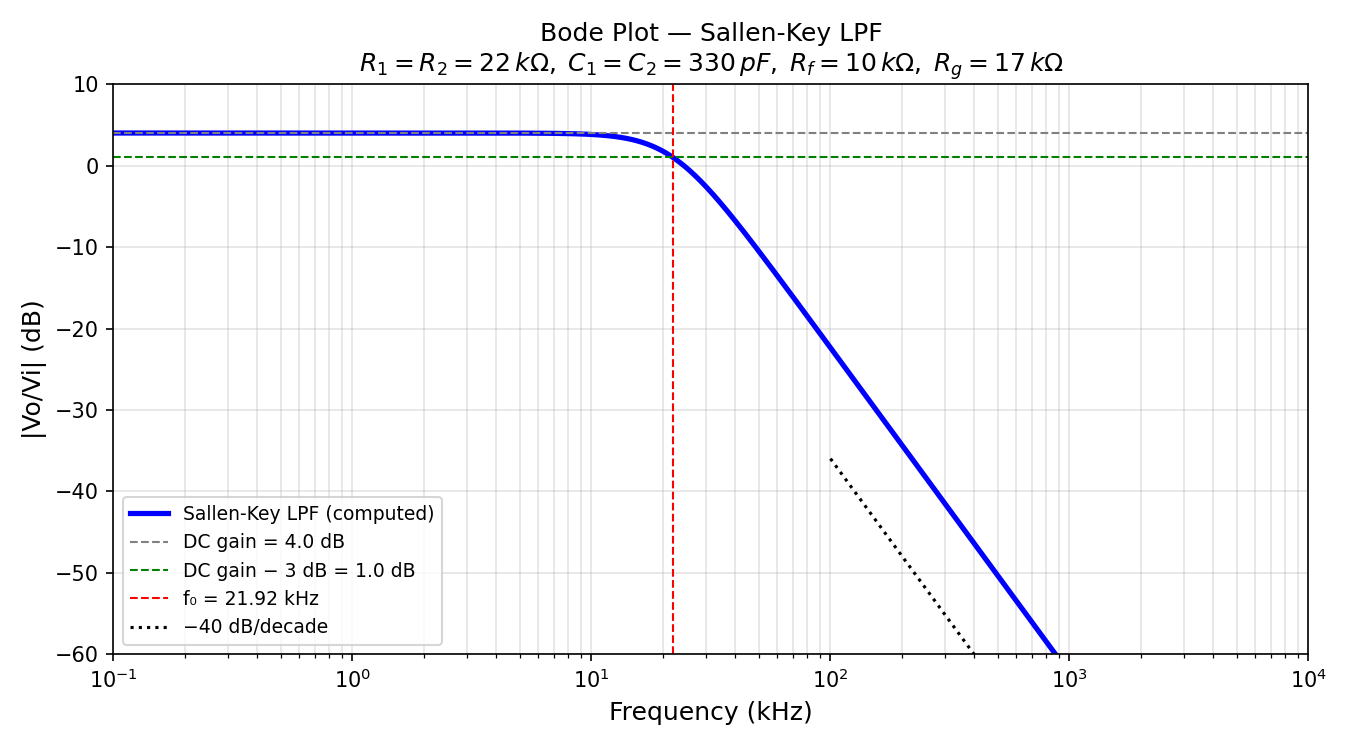
\includegraphics[width=1\linewidth]{image/bode_1_1_52}
	\caption{}
	\label{fig:bode1152}
\end{figure}
\end{frame}
\begin{frame}[fragile]{Python Verification — Parameters \& Transfer Function}
	\begin{lstlisting}[language=Python, basicstyle=\tiny\ttfamily,
		keywordstyle=\color{blue}, commentstyle=\color{gray},
		stringstyle=\color{orange}, breaklines=true]
		import numpy as np
		import matplotlib.pyplot as plt
		from scipy import signal
		
		# Parameters
		R  = 22e3;   C  = 330e-12     # Ohm, F
		Rf = 10e3;   Rg = 17e3        # Ohm
		
		K  = 1 + Rf / Rg
		w0 = 1 / (R * C)
		f0 = w0 / (2 * np.pi)
		Q  = 1 / (3 - K)
		
		print(f"K      = {K:.6f}  ({20*np.log10(K):.2f} dB)")
		print(f"f0     = {f0/1e3:.3f} kHz")
		print(f"omega0 = {w0:.2f} rad/s")
		print(f"Q      = {Q:.4f}  (1/sqrt(2) = {1/np.sqrt(2):.4f})")
		print(f"Filter : {'Butterworth' if abs(Q - 1/np.sqrt(2)) < 0.01 else 'Other'}")
		
		# Transfer function: H(s) = K*w0^2 / (s^2 + w0*(3-K)*s + w0^2)
		num = [K * w0**2]
		den = [1, w0 * (3 - K), w0**2]
	\end{lstlisting}
\end{frame}

\begin{frame}[fragile]{Python Verification — Bode Plot}
	\begin{lstlisting}[language=Python, basicstyle=\tiny\ttfamily,
		keywordstyle=\color{blue}, commentstyle=\color{gray},
		stringstyle=\color{orange}, breaklines=true]
		f = np.logspace(2, 7, 2000)
		w = 2 * np.pi * f
		_, H = signal.freqs(num, den, worN=w)
		mag_dB = 20 * np.log10(np.abs(H))
		
		fig, ax = plt.subplots(figsize=(9, 5))
		ax.semilogx(f / 1e3, mag_dB, 'b-', lw=2.5, label='Sallen-Key LPF (computed)')
		ax.axhline(20*np.log10(K),     color='gray',  ls='--', lw=1, label=f'DC gain = {20*np.log10(K):.1f} dB')
		ax.axhline(20*np.log10(K) - 3, color='green', ls='--', lw=1, label=f'DC gain - 3 dB = {20*np.log10(K)-3:.1f} dB')
		ax.axvline(f0 / 1e3,           color='red',   ls='--', lw=1, label=f'f0 = {f0/1e3:.2f} kHz')
		
		f_slope = np.array([1e5, 1e6])
		ref_dB  = 20 * np.log10(K) - 40
		ax.semilogx(f_slope/1e3, [ref_dB, ref_dB-40], 'k:', lw=1.5, label='-40 dB/decade')
		
		ax.set_xlabel('Frequency (kHz)');  ax.set_ylabel('|Vo/Vi| (dB)')
		ax.set_xlim([0.1, 1e4]);           ax.set_ylim([-60, 10])
		ax.legend(fontsize=9);             ax.grid(True, which='both', alpha=0.35)
		plt.tight_layout();                plt.savefig('bode_1_1_52.png', dpi=150)
		
		# Verify gain at f0
		_, H_at_f0 = signal.freqs(num, den, worN=[w0])
		print(f"Gain at f0: {20*np.log10(abs(H_at_f0[0])):.3f} dB  "
		f"(expected {20*np.log10(K)-3:.3f} dB)")
	\end{lstlisting}
\end{frame}

\end{document}
	